% vim: set spell
% vim: spelllang=en
\PassOptionsToPackage{unicode}{hyperref}
\documentclass[aspectratio=1610, 9pt]{beamer}

\usetheme{vertex}


\setmathfont{XITS Math}[range={cal, bfcal}]

\usepackage[main=german, english]{babel}
\usepackage[autostyle]{csquotes}

\usepackage{xcolor}

\usepackage{tcolorbox}
\usepackage[]{siunitx}
\setmathfont{Fira Math}
\AtBeginDocument{\sisetup{math-rm=\mathrm,math-micro=μ}}

\usepackage{graphicx}
\usepackage{tikz}
\usepackage{calc}

% \usepackage{biblatex}

\usepackage{hyperref}
\usepackage{bookmark}

\usepackage{xparse}
\usepackage{expl3}

\NewDocumentCommand \TT {} {\ensuremath{\operatorname{TT}}}
\NewDocumentCommand \TAI {} {\ensuremath{\operatorname{TAI}}}
\NewDocumentCommand \UT {} {\ensuremath{\operatorname{UT1}}}
\NewDocumentCommand \UTC {} {\ensuremath{\operatorname{UTC}}}

\RenewDocumentCommand \d {m} {\TextOrMath{\textd{#1}}{\mathinner{\symup{d}#1}}}

\NewDocumentCommand \heading {m} {{%
  \textcolor{vertexDarkRed}{\bfseries\large #1}
  \par\medskip%
}}


\title{Celestial Coordinates}%

\author[M. Nöthe]{Maximilian Nöthe}
\date[2020-10-09]{Group Seminar 2020-10-09}
\institute[E5b]{
\includegraphics[height=0.1\textheight]{logos/e5b.pdf}}

\begin{document}

\maketitle

\begin{frame}[c]{Overview}
 \tableofcontents
\end{frame}

\begin{frame}{Where do I need to point my telescope}
\end{frame}

\section{Time}
\bumper{Time}

\begin{frame}{The Two Concepts of Time}
  \begin{columns}[t, onlytextwidth]
    \begin{column}{0.475\textwidth}
      \begin{center}
        \heading{Earth's Orientation}
        \only<1>{%
          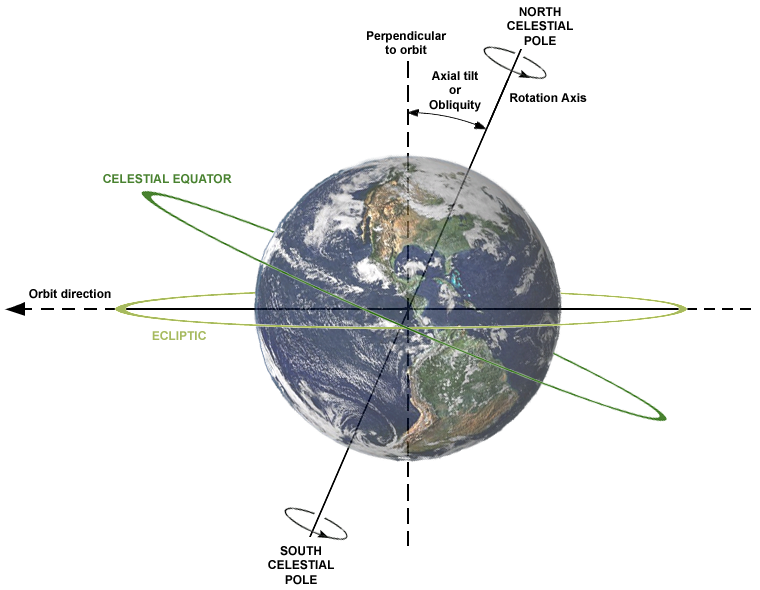
\includegraphics[height=3.5cm]{images/AxialTiltObliquity.png}\\[-1.2\baselineskip]
          \hspace{2.5cm}{\small[Dna-Dennis]}
        }%
        \only<2->{%
          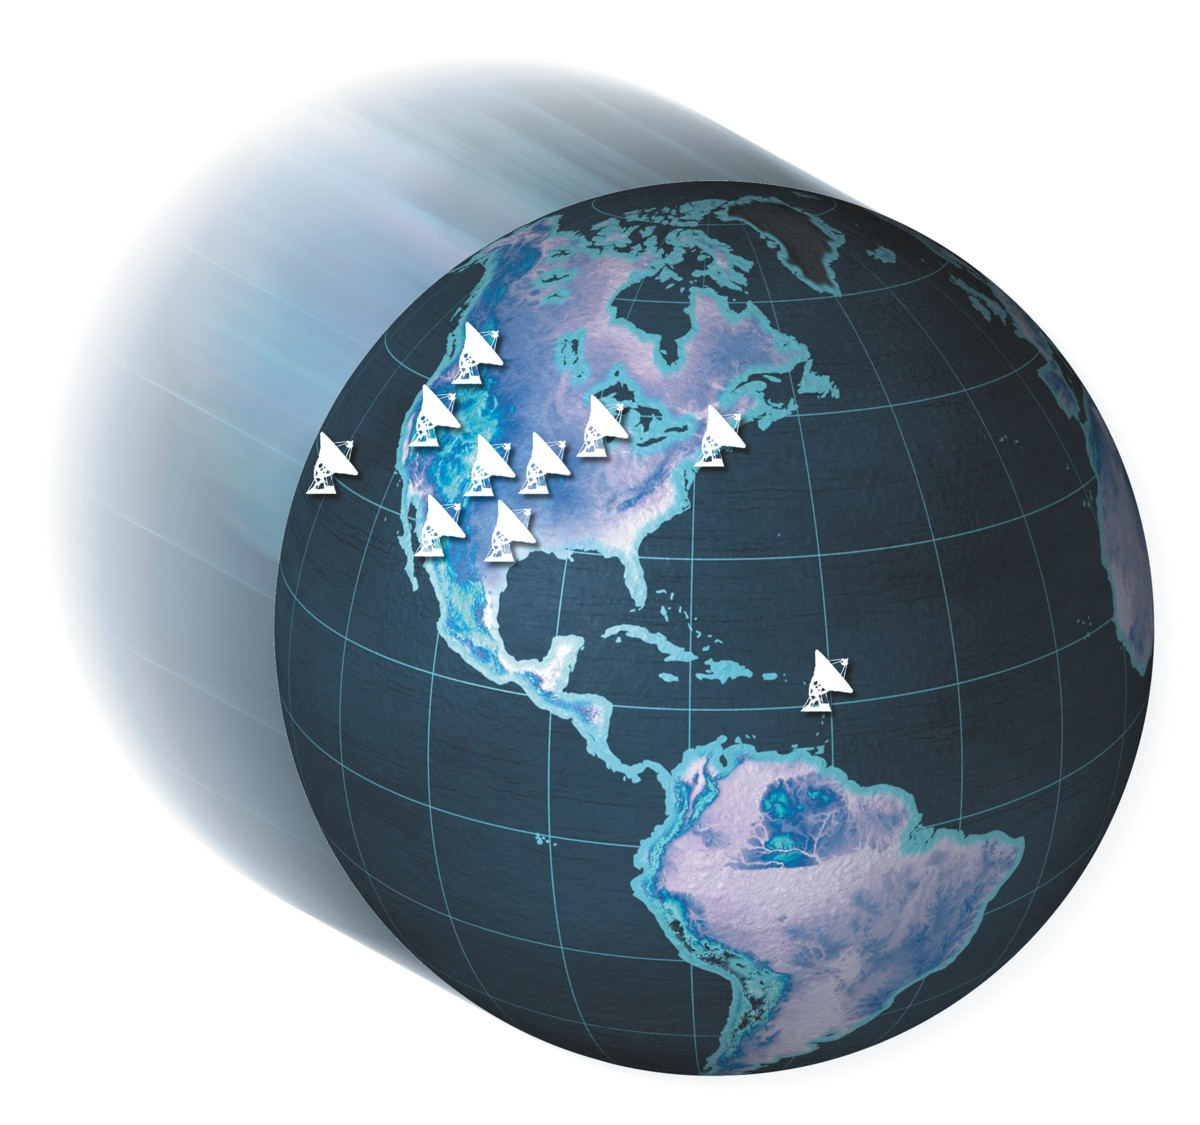
\includegraphics[height=3.5cm]{images/vlba.jpeg}\\[-1.2\baselineskip]
          \hspace{-3.5cm}{\small[NASA]}
        }%
      \end{center}

      \begin{itemize}
        \item The historical concept
        \item Base of calendars $⇒ $ leap years
      \end{itemize}
    \end{column}
    \begin{column}{0.525\textwidth}
      \onslide<3->{
        \begin{center}
          \heading{Linear Time}
          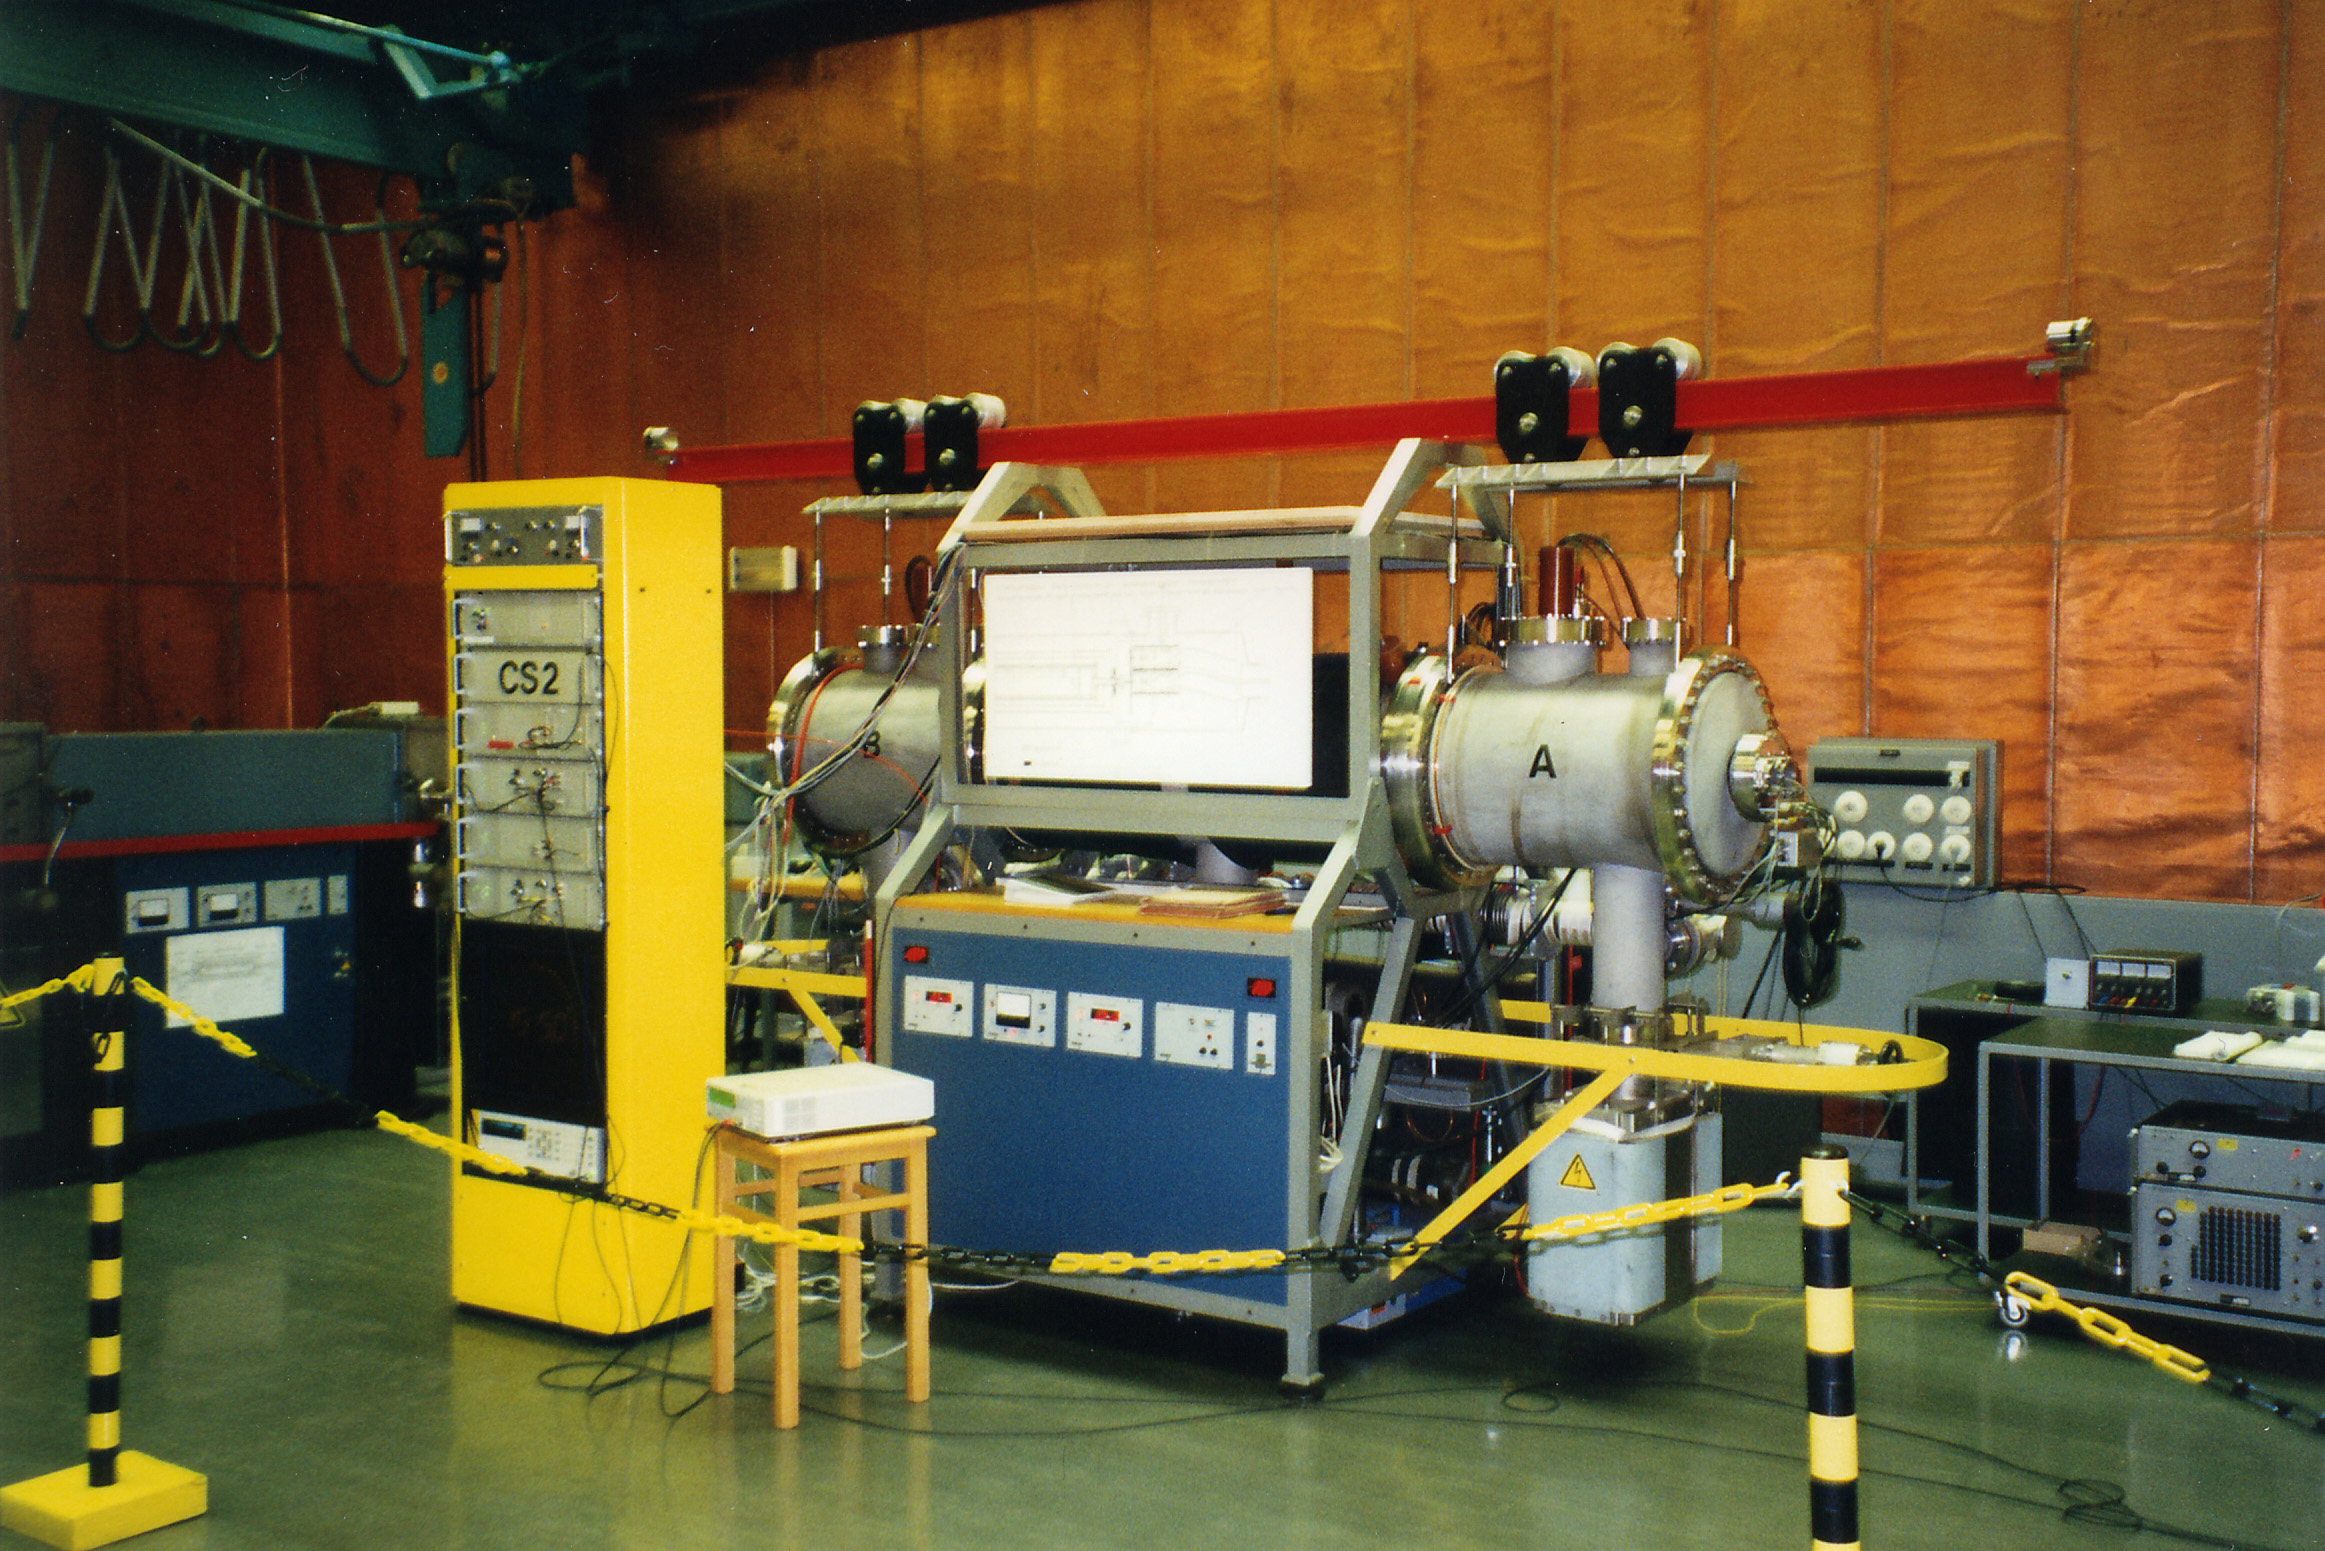
\includegraphics[height=3.5cm]{images/Atomuhr-CS2.jpg}\\[-1.2\baselineskip]
          \hspace{3.5cm}{\color{black!20}\small[Jörg Behrens]}
        \end{center}

        \begin{itemize}
          \item Based on clocks
          \item Monotonically ticking SI seconds
        \end{itemize}
      }
    \end{column}
  \end{columns}
  \medskip
  \begin{columns}[t, onlytextwidth]
    \begin{column}{0.475\textwidth}
      \onslide<2->{%
        \begin{center}
          \large\bfseries
          Measured daily by radio telescopes\\ (e.\,g.\ by the VLBA)
        \end{center}
      }
    \end{column}
    \hfill
    \begin{column}{0.525\textwidth}
      \onslide<4->{%
        \begin{center}
          \large\bfseries
          Measured by atomic clocks\\
        \end{center}
      }
    \end{column}
  \end{columns}
\end{frame}

\begin{frame}{Time Standards}
  \framesubtitle{UT1, ERA, TAI, TT}
  \begin{columns}[t, onlytextwidth]
    \begin{column}{0.495\textwidth}
      \begin{center}
        \heading{Earth's Orientation}

        \begin{description}[ERA $(\theta)$]
          \item[UT1] Universal Time 1
            \begin{itemize}
              \item Measured daily by VLBI
              \item Units have variable length, since $\SI{1}{\day} = \SI{24}{\hour} = \SI{1440}{\minute} = \SI{86400}{\second}$
              \item Can only be known in hindsight
              \item Published as $\increment(\operatorname{UT1}, \operatorname{UTC})$ tables
            \end{itemize}
          \item[ERA ($\theta$)] Earth Orientation Angle \\
            UT1 expressed as angle
        \end{description}
      \end{center}
    \end{column}
    \begin{column}{0.495\textwidth}
      \begin{center}
      \heading{Linear Time}
        \begin{description}[TAI]
          \item[TAI] Temps Atomique International
            \begin{itemize}
              \item Maintained by the BIPM
              \item Uses $>600$ atomic clocks in 60 institutes
              \item Preliminary \TAI{} time broadcast
              \item Final \TAI{} published monthly
              \item SI seconds on Earth's Geoid\\ → relativistic corrections
            \end{itemize}
          \item[TT] Terrestrial Time
            \begin{itemize}
              \item Idealised timescale for time on Earth's Geoid
              \item Realized as $\TT(\TAI) = \TAI{} + \SI{32.184}{\second}$
            \end{itemize}
        \end{description}
      \end{center}
    \end{column}
  \end{columns}
\end{frame}

\begin{frame}[c]{Time Standards}
  \framesubtitle{UTC}
  \begin{columns}[c, onlytextwidth]
    \begin{column}{0.5\textwidth}
      \centering
      \textbf{\Large Bit of Both}\\[0.5\baselineskip]%
      \begin{description}[UTC]
        \item[UTC] Coordinated Universal Time
        \begin{itemize}
          \item Civil Timekeeping
          \item Based on \TAI
          \item Difference to \UT{} kept $<\SI{1}{\second}$ by leapseconds \\
            \texttt{2020-12-31T23:59:60}
          \item Currently: $\UTC = \TAI - \SI{37}{\second}$
        \end{itemize}
      \end{description}
    \end{column}
    \hfill
    \begin{column}{0.5\textwidth}
      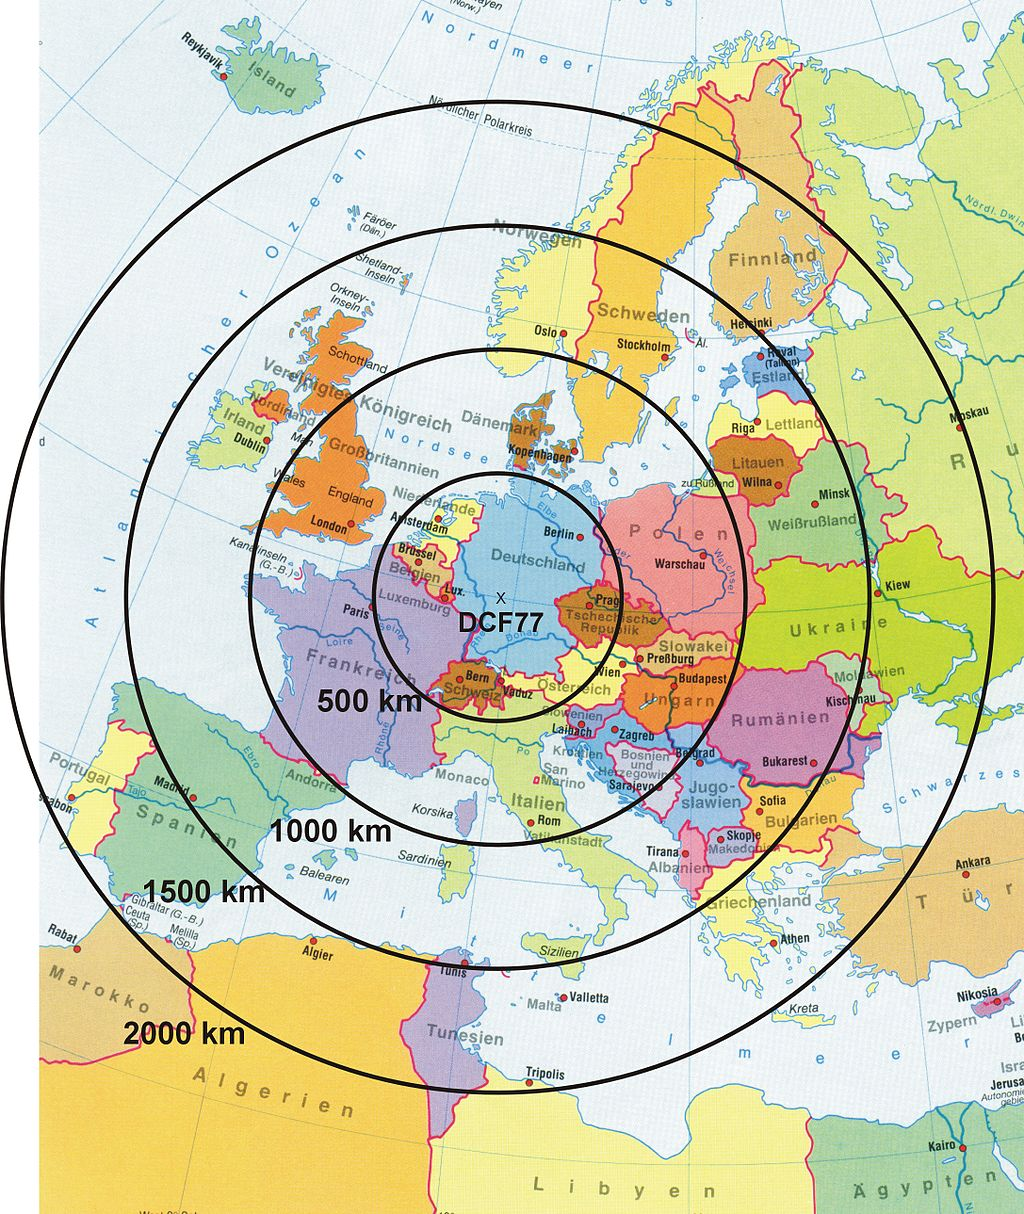
\includegraphics[height=0.9\textheight]{images/dcf77.jpg}\\[-1.2\baselineskip]
      \hspace{2em}[PTB (Erika Schow)]
    \end{column}
  \end{columns}
\end{frame}

\section{Terrestrial Coordinates}
\bumper{Terrestrial Coordinates}

\begin{frame}{International Terrestrial References System and Frames}

  The ITRS is defined by axis fixed on the Earth's crust with no net rotation
  through continental drift

  \begin{description}[$(0,0,0)$]
    \item[$\color{vertexDarkRed} z$-Axis] Earth's rotation axis
    \item[$\color{vertexDarkRed} x$-Axis] in the equatorial plane through the 0 meridian
    \item[$\color{vertexDarkRed} y$-Axis] perpendicular to $x$ and $z$ form a right handed system
    \item[$\color{vertexDarkRed} (0, 0, 0)$] Earth's barycenter
  \end{description}

  We mostly use spherical coordinates: latitude, longitude and height above
  the reference geoid.

  \bigskip

  A reference frame is an implementation of a reference system based on ground stations:

  \begin{itemize}
    \item GPS (Global Positioning System) / Galileo ground stations
    \item VLBI telescopes
    \item Satellite laser ranging
    \item DORIS (Doppler Orbitography and Radiopositioning Integrated by Satellite)
  \end{itemize}
\end{frame}

\begin{frame}[t]{ITRF / WGS84}
  \centering
  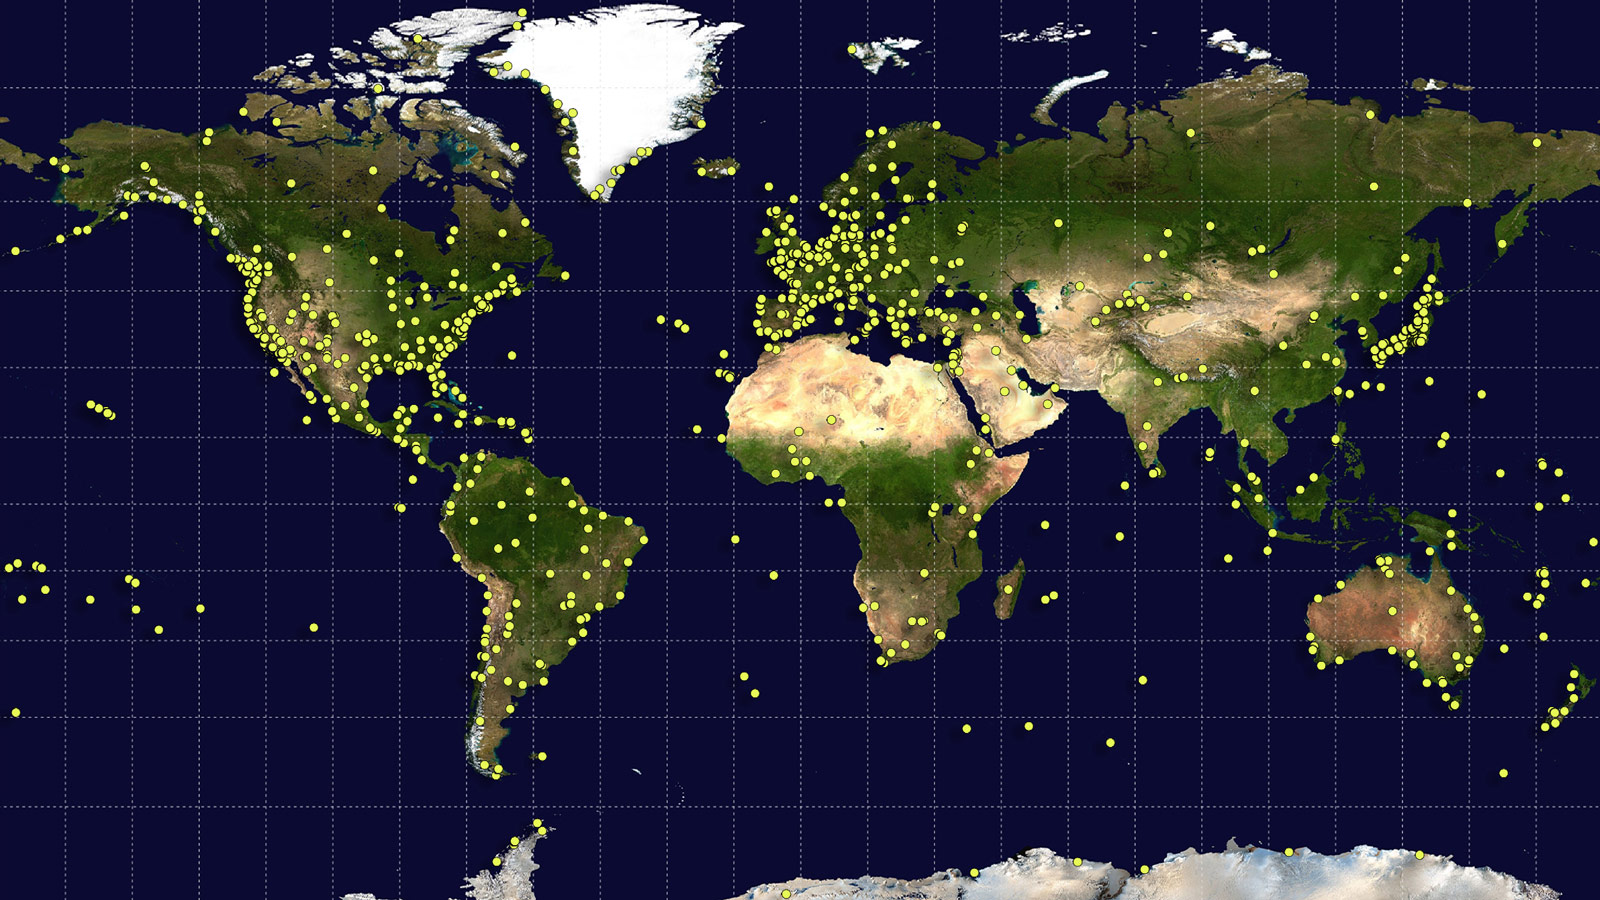
\includegraphics[
    width=\textwidth,
    height=0.9\textheight,
    keepaspectratio
  ]{images/itrf_groundstations.jpg}\\[-3\baselineskip]
  \textcolor{white}{[NASA/Earth Observatory/GSFC]}\\[2\baselineskip]

  Two main reference frames today: WGS84 and ITRF. Difference only centimeters.
\end{frame}

\section{Precession / Nutation / Polar Motion}
\bumper{Precession / Nutation / Polar Motion}

\begin{frame}{title}
\end{frame}

\section{The Fundamental Celestial Reference System}
\begin{frame}{title}
\end{frame}

\section{Equatorial Coordinates}
\begin{frame}{title}
\end{frame}

\section{Horizontal Coordinates}
\begin{frame}{title}
\end{frame}

\section{Galactic Coordinates}
\begin{frame}{title}
\end{frame}

\section{Using \texttt{astropy} for Coordinate Transformation}
\bumper{Never do live demo}

\end{document}
